\documentclass{standalone}
\usepackage{tikz}
\usetikzlibrary{patterns, positioning}

\begin{document}
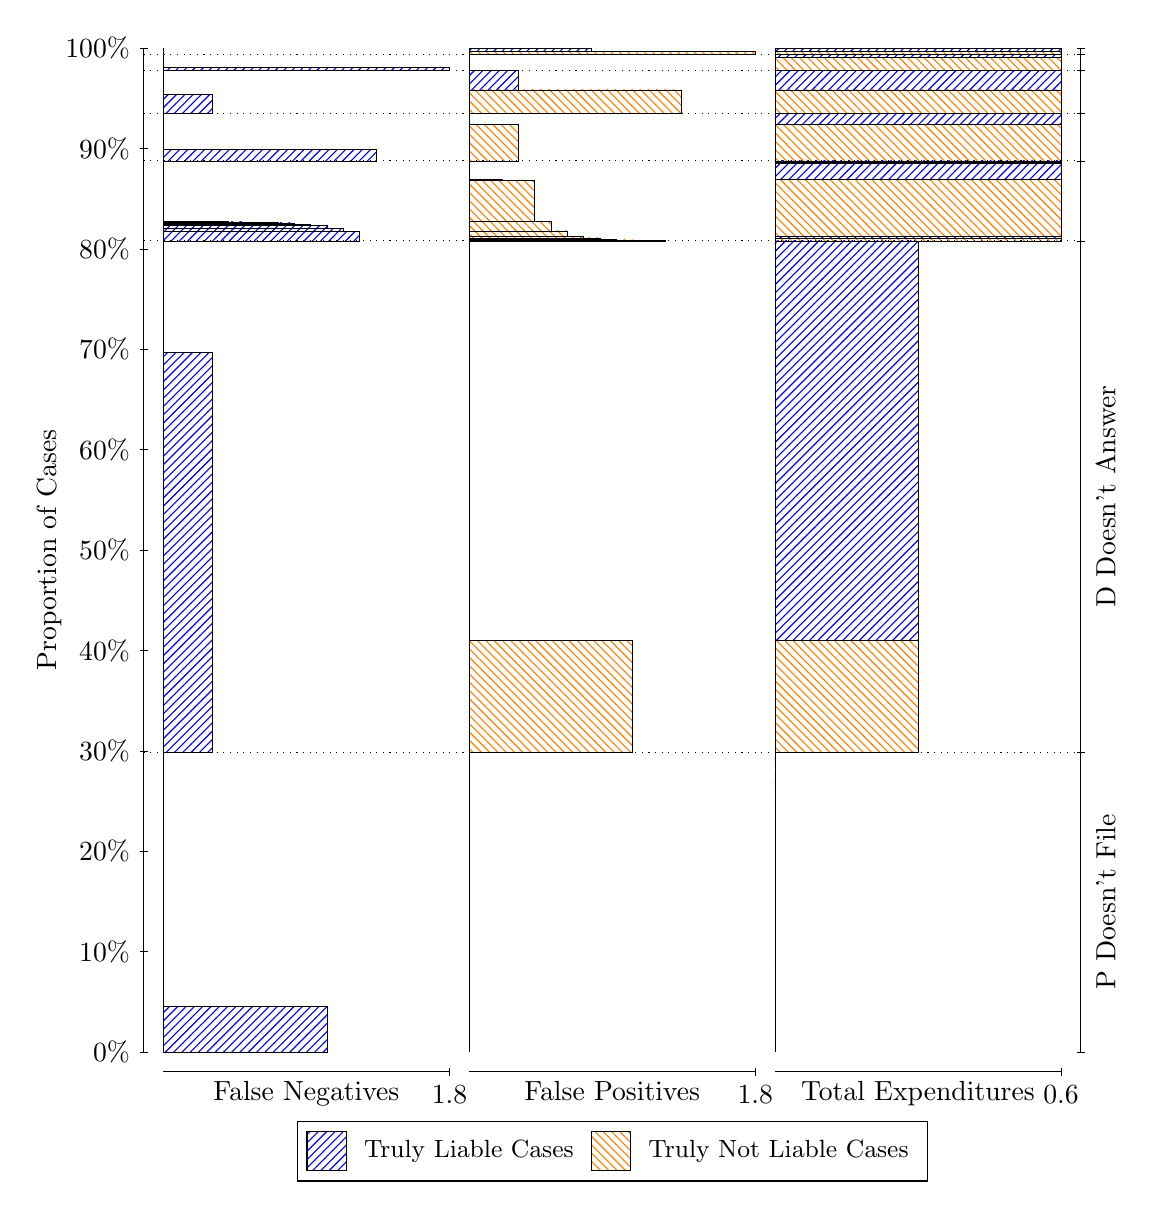
\begin{tikzpicture}
\draw[black, very thin] (1.5,1.75) -- (1.5,14.5);
\node[rotate=90, anchor=center] at (0.3, 8.125) {Proportion of Cases};
\draw[black, very thin] (1.45,1.75) -- (1.55,1.75);
\node[anchor=east] at (1.45, 1.75) {0\%};
\draw[black, very thin] (1.45,3.025) -- (1.55,3.025);
\node[anchor=east] at (1.45, 3.025) {10\%};
\draw[black, very thin] (1.45,4.3) -- (1.55,4.3);
\node[anchor=east] at (1.45, 4.3) {20\%};
\draw[black, very thin] (1.45,5.575) -- (1.55,5.575);
\node[anchor=east] at (1.45, 5.575) {30\%};
\draw[black, very thin] (1.45,6.85) -- (1.55,6.85);
\node[anchor=east] at (1.45, 6.85) {40\%};
\draw[black, very thin] (1.45,8.125) -- (1.55,8.125);
\node[anchor=east] at (1.45, 8.125) {50\%};
\draw[black, very thin] (1.45,9.4) -- (1.55,9.4);
\node[anchor=east] at (1.45, 9.4) {60\%};
\draw[black, very thin] (1.45,10.675) -- (1.55,10.675);
\node[anchor=east] at (1.45, 10.675) {70\%};
\draw[black, very thin] (1.45,11.95) -- (1.55,11.95);
\node[anchor=east] at (1.45, 11.95) {80\%};
\draw[black, very thin] (1.45,13.225) -- (1.55,13.225);
\node[anchor=east] at (1.45, 13.225) {90\%};
\draw[black, very thin] (1.45,14.5) -- (1.55,14.5);
\node[anchor=east] at (1.45, 14.5) {100\%};

\draw[black, very thin] (13.4,1.75) -- (13.4,14.5);
\draw[black, very thin] (13.35,1.75) -- (13.45,1.75);
\node[anchor=west] at (13.35, 1.75) {};
\draw[black, very thin] (13.35,5.5578) -- (13.45,5.5578);
\node[anchor=west] at (13.35, 5.5578) {};
\draw[black, very thin] (13.35,12.052) -- (13.45,12.052);
\node[anchor=west] at (13.35, 12.052) {};
\draw[black, very thin] (13.35,13.067) -- (13.45,13.067);
\node[anchor=west] at (13.35, 13.067) {};
\draw[black, very thin] (13.35,13.667) -- (13.45,13.667);
\node[anchor=west] at (13.35, 13.667) {};
\draw[black, very thin] (13.35,14.214) -- (13.45,14.214);
\node[anchor=west] at (13.35, 14.214) {};
\draw[black, very thin] (13.35,14.415) -- (13.45,14.415);
\node[anchor=west] at (13.35, 14.415) {};
\draw[black, very thin] (13.35,14.5) -- (13.45,14.5);
\node[anchor=west] at (13.35, 14.5) {};

\draw[black, very thin, pattern color=blue, pattern=north east lines] (1.75,1.75) rectangle (3.8262,2.3308);
\draw[black, very thin, pattern color=orange, pattern=north west lines] (1.75,2.3308) rectangle (1.75,5.5578);
\draw[black, very thin, pattern color=blue, pattern=north east lines] (1.75,5.5578) rectangle (2.3729,10.636);
\draw[black, very thin, pattern color=orange, pattern=north west lines] (1.75,10.636) rectangle (1.75,12.052);
\draw[black, very thin, pattern color=blue, pattern=north east lines] (1.75,12.052) rectangle (4.2414,12.173);
\draw[black, very thin, pattern color=blue, pattern=north east lines] (1.75,12.173) rectangle (4.0338,12.213);
\draw[black, very thin, pattern color=blue, pattern=north east lines] (1.75,12.213) rectangle (3.8262,12.249);
\draw[black, very thin, pattern color=blue, pattern=north east lines] (1.75,12.249) rectangle (3.6186,12.254);
\draw[black, very thin, pattern color=blue, pattern=north east lines] (1.75,12.254) rectangle (3.6186,12.262);
\draw[black, very thin, pattern color=blue, pattern=north east lines] (1.75,12.262) rectangle (3.411,12.278);
\draw[black, very thin, pattern color=blue, pattern=north east lines] (1.75,12.278) rectangle (3.2033,12.283);
\draw[black, very thin, pattern color=blue, pattern=north east lines] (1.75,12.283) rectangle (2.9957,12.29);
\draw[black, very thin, pattern color=blue, pattern=north east lines] (1.75,12.29) rectangle (2.7881,12.292);
\draw[black, very thin, pattern color=blue, pattern=north east lines] (1.75,12.292) rectangle (2.5805,12.296);
\draw[black, very thin, pattern color=orange, pattern=north west lines] (1.75,12.296) rectangle (1.75,13.067);
\draw[black, very thin, pattern color=blue, pattern=north east lines] (1.75,13.067) rectangle (4.449,13.208);
\draw[black, very thin, pattern color=orange, pattern=north west lines] (1.75,13.208) rectangle (1.75,13.667);
\draw[black, very thin, pattern color=blue, pattern=north east lines] (1.75,13.667) rectangle (2.3729,13.912);
\draw[black, very thin, pattern color=orange, pattern=north west lines] (1.75,13.912) rectangle (1.75,14.214);
\draw[black, very thin, pattern color=blue, pattern=north east lines] (1.75,14.214) rectangle (5.3833,14.252);
\draw[black, very thin, pattern color=orange, pattern=north west lines] (1.75,14.252) rectangle (1.75,14.415);
\draw[black, very thin, pattern color=orange, pattern=north west lines] (1.75,14.415) rectangle (1.75,14.453);
\draw[black, very thin, pattern color=blue, pattern=north east lines] (1.75,14.453) rectangle (1.75,14.5);
\draw[black, very thin, pattern color=orange, pattern=north west lines] (5.6333,1.75) rectangle (5.6333,4.977);
\draw[black, very thin, pattern color=blue, pattern=north east lines] (5.6333,4.977) rectangle (5.6333,5.5578);
\draw[black, very thin, pattern color=orange, pattern=north west lines] (5.6333,5.5578) rectangle (7.7095,6.9733);
\draw[black, very thin, pattern color=blue, pattern=north east lines] (5.6333,6.9733) rectangle (5.6333,12.052);
\draw[black, very thin, pattern color=orange, pattern=north west lines] (5.6333,12.052) rectangle (8.1248,12.054);
\draw[black, very thin, pattern color=orange, pattern=north west lines] (5.6333,12.054) rectangle (7.9171,12.056);
\draw[black, very thin, pattern color=orange, pattern=north west lines] (5.6333,12.056) rectangle (7.7095,12.062);
\draw[black, very thin, pattern color=orange, pattern=north west lines] (5.6333,12.062) rectangle (7.5019,12.069);
\draw[black, very thin, pattern color=orange, pattern=north west lines] (5.6333,12.069) rectangle (7.2943,12.088);
\draw[black, very thin, pattern color=orange, pattern=north west lines] (5.6333,12.088) rectangle (7.0867,12.104);
\draw[black, very thin, pattern color=orange, pattern=north west lines] (5.6333,12.104) rectangle (6.879,12.177);
\draw[black, very thin, pattern color=orange, pattern=north west lines] (5.6333,12.177) rectangle (6.6714,12.296);
\draw[black, very thin, pattern color=orange, pattern=north west lines] (5.6333,12.296) rectangle (6.4638,12.823);
\draw[black, very thin, pattern color=blue, pattern=north east lines] (5.6333,12.823) rectangle (6.0486,12.827);
\draw[black, very thin, pattern color=blue, pattern=north east lines] (5.6333,12.827) rectangle (5.841,12.829);
\draw[black, very thin, pattern color=blue, pattern=north east lines] (5.6333,12.829) rectangle (5.6333,13.067);
\draw[black, very thin, pattern color=orange, pattern=north west lines] (5.6333,13.067) rectangle (6.2562,13.526);
\draw[black, very thin, pattern color=blue, pattern=north east lines] (5.6333,13.526) rectangle (5.6333,13.667);
\draw[black, very thin, pattern color=orange, pattern=north west lines] (5.6333,13.667) rectangle (8.3324,13.969);
\draw[black, very thin, pattern color=blue, pattern=north east lines] (5.6333,13.969) rectangle (6.2562,14.214);
\draw[black, very thin, pattern color=orange, pattern=north west lines] (5.6333,14.214) rectangle (5.6333,14.377);
\draw[black, very thin, pattern color=blue, pattern=north east lines] (5.6333,14.377) rectangle (5.6333,14.415);
\draw[black, very thin, pattern color=orange, pattern=north west lines] (5.6333,14.415) rectangle (9.2667,14.453);
\draw[black, very thin, pattern color=blue, pattern=north east lines] (5.6333,14.453) rectangle (7.1905,14.5);
\draw[black, very thin, pattern color=orange, pattern=north west lines] (9.5167,1.75) rectangle (9.5167,4.977);
\draw[black, very thin, pattern color=blue, pattern=north east lines] (9.5167,4.977) rectangle (9.5167,5.5578);
\draw[black, very thin, pattern color=orange, pattern=north west lines] (9.5167,5.5578) rectangle (11.333,6.9733);
\draw[black, very thin, pattern color=blue, pattern=north east lines] (9.5167,6.9733) rectangle (11.333,12.052);
\draw[black, very thin, pattern color=orange, pattern=north west lines] (9.5167,12.052) rectangle (13.15,12.078);
\draw[black, very thin, pattern color=blue, pattern=north east lines] (9.5167,12.078) rectangle (13.15,12.103);
\draw[black, very thin, pattern color=orange, pattern=north west lines] (9.5167,12.103) rectangle (13.15,12.829);
\draw[black, very thin, pattern color=blue, pattern=north east lines] (9.5167,12.829) rectangle (13.15,13.031);
\draw[black, very thin, pattern color=orange, pattern=north west lines] (9.5167,13.031) rectangle (13.15,13.049);
\draw[black, very thin, pattern color=blue, pattern=north east lines] (9.5167,13.049) rectangle (13.15,13.067);
\draw[black, very thin, pattern color=orange, pattern=north west lines] (9.5167,13.067) rectangle (13.15,13.526);
\draw[black, very thin, pattern color=blue, pattern=north east lines] (9.5167,13.526) rectangle (13.15,13.667);
\draw[black, very thin, pattern color=orange, pattern=north west lines] (9.5167,13.667) rectangle (13.15,13.969);
\draw[black, very thin, pattern color=blue, pattern=north east lines] (9.5167,13.969) rectangle (13.15,14.214);
\draw[black, very thin, pattern color=orange, pattern=north west lines] (9.5167,14.214) rectangle (13.15,14.377);
\draw[black, very thin, pattern color=blue, pattern=north east lines] (9.5167,14.377) rectangle (13.15,14.415);
\draw[black, very thin, pattern color=orange, pattern=north west lines] (9.5167,14.415) rectangle (13.15,14.453);
\draw[black, very thin, pattern color=blue, pattern=north east lines] (9.5167,14.453) rectangle (13.15,14.5);
\draw[black, dotted] (1.5,5.5578) -- (13.4,5.5578);
\draw[black, dotted] (1.5,12.052) -- (13.4,12.052);
\draw[black, dotted] (1.5,13.067) -- (13.4,13.067);
\draw[black, dotted] (1.5,13.667) -- (13.4,13.667);
\draw[black, dotted] (1.5,14.214) -- (13.4,14.214);
\draw[black, dotted] (1.5,14.415) -- (13.4,14.415);
\draw[black, very thin] (1.75,1.5) -- (5.3833,1.5);
\node[anchor=north] at (3.5667, 1.5) {False Negatives};
\draw[black, very thin] (5.3833,1.45) -- (5.3833,1.55);
\node[anchor=north] at (5.3833, 1.45) {1.8};

\draw[black, very thin] (5.6333,1.5) -- (9.2667,1.5);
\node[anchor=north] at (7.45, 1.5) {False Positives};
\draw[black, very thin] (9.2667,1.45) -- (9.2667,1.55);
\node[anchor=north] at (9.2667, 1.45) {1.8};

\draw[black, very thin] (9.5167,1.5) -- (13.15,1.5);
\node[anchor=north] at (11.333, 1.5) {Total Expenditures};
\draw[black, very thin] (13.15,1.45) -- (13.15,1.55);
\node[anchor=north] at (13.15, 1.45) {0.6};

\node[black, centered, rotate=90] at (13.72, 3.6539) {P Doesn't File};
\node[black, centered, rotate=90] at (13.72, 8.8048) {D Doesn't Answer};






\draw (7.449999999999999,1.5) node[draw=none] (baseCoordinate) {};
\begin{scope}[align=center]
        \matrix[scale=0.5, draw=black, below=0.5cm of baseCoordinate, nodes={draw}, column sep=0.1cm]{
            \node[rectangle, draw, minimum width=0.5cm, minimum height=0.5cm, pattern=north east lines, pattern color=blue] {}; &
            \node[draw=none, font=\small] (B) {Truly Liable Cases}; &
            \node[rectangle, draw, minimum width=0.5cm, minimum height=0.5cm, pattern=north west lines, pattern color=orange] {}; &
            \node[draw=none, font=\small] (B) {Truly Not Liable Cases}; \\
            };
\end{scope}

\end{tikzpicture}
\end{document}